\section{1174086 – Tia Nur Candida}
    \subsection{Teori}
        \begin{enumerate}
            \item Jelaskan dengan ilustrasi gambar sendiri apa itu generator dengan perumpamaan anda sebagai mahasiswa sebagai generatornya.
            \par Generator adalah sebuah jaringan yang merubah inputan vektor menjadi gambar, seperti ada inputan vektor secara acak yaitu angka sembarang, maka angka tersebut akan diubah menjadi gambar yang sembarang pula. Sebagai ilustrasi apabila mahasiswa sebagai generator, mmisalkan inputan vektor tersebut adalah bahan bahan membuat kue, maka hasil dari generator tersebut juga akan acak, bisa kue bolu, cupcake, ataupun kue lainnya.
            \begin{figure}[H]
                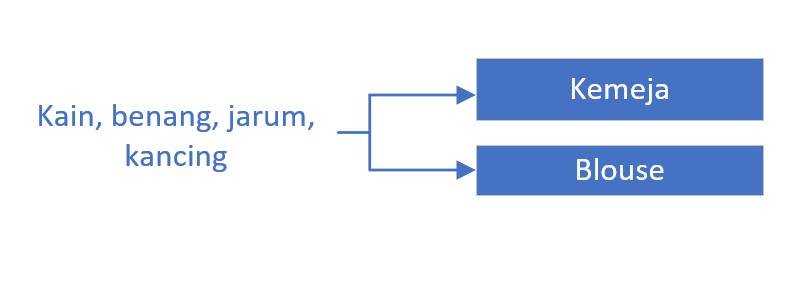
\includegraphics[width=4cm]{figures/1174086/chapter8/teori1.png}
                \centering
                  \caption{Teori No 1}
            \end{figure}

            \item Jelaskan dengan ilustrasi gambar sendiri apa itu diskriminator dengan perumpamaan dosen anda sebagai diskriminatornya
            \par Diskriminator adalah sebuah jaringan yang mengeluarkan klasifikasi untuk menyatakan input gambar adalah asli dari dataset atau buatan dari generator. Lebih mudahnya diskriminator digunakan agar hasil gambar dari generator sesuai dengan yang diinginkan. sebagai ilustrasi nya dosen menyuruh mahasiswanya membuat kue bolu, maka hasil yang akan dibuat adalah kue bolu.
            \begin{figure}[H]
                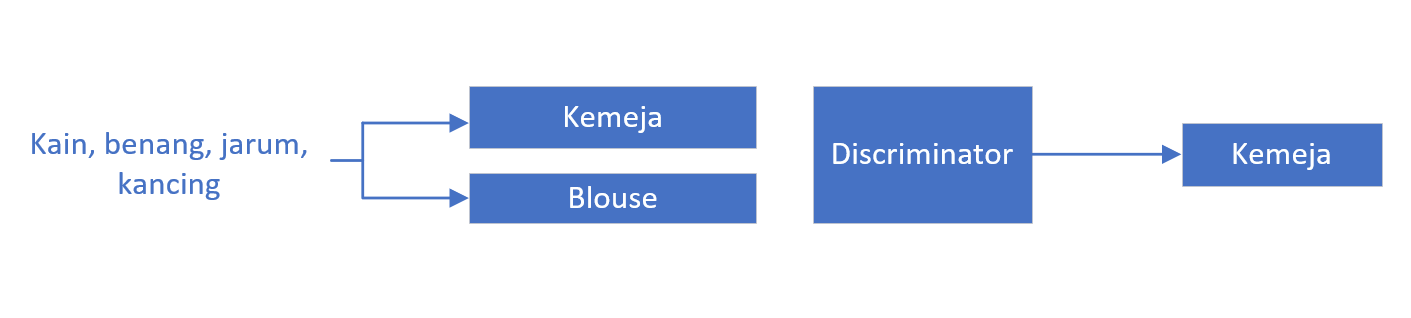
\includegraphics[width=4cm]{figures/1174086/chapter8/teori2.png}
                \centering
                  \caption{Teori No 2}
            \end{figure}

            \item Jelaskan dengan ilustrasi gambar sendiri bagaimana arsitektur generator dibua
            \par Generator menggunkan input array random yang bernama seed, dimana akan diubah menjadi sebuah gambar dengan menggunakan Convolutional Neural Network yang dapat dilihat pada gambar.
            \begin{figure}[H]
                
\includegraphics[width=4cm]{figures/1174086/chapter8/teori3.png}
                \centering
                  \caption{Teori No 3}
            \end{figure}

            \item Jelaskan dengan ilustrasi gambar sendiri bagaimana arsitektur diskriminator dibuat
            \par Diskriminator adalah CNN yang menerima inputan image lalu menghasilkan angka biner yang dapat menyatakan apakah gambar tersebut asli atau sesuai dengan dataset asli
            \begin{figure}[H]
                
\includegraphics[width=4cm]{figures/1174086/chapter8/teori4.png}
                \centering
                  \caption{Teori No 4}
            \end{figure}

            \item Jelaskan dengan ilustrasi gambar apa itu latent space
            \par latent space adalah representasi dari data yang di kompress, untuk contohnya misalnya ada 3 gambar yaitu 2 kursi yang berebeda dan 1 meja, maka hal hal yang mirip dai kursi tersebut(ciri-ciri utamanya), seeprti itulah latent space
            \begin{figure}[H]
                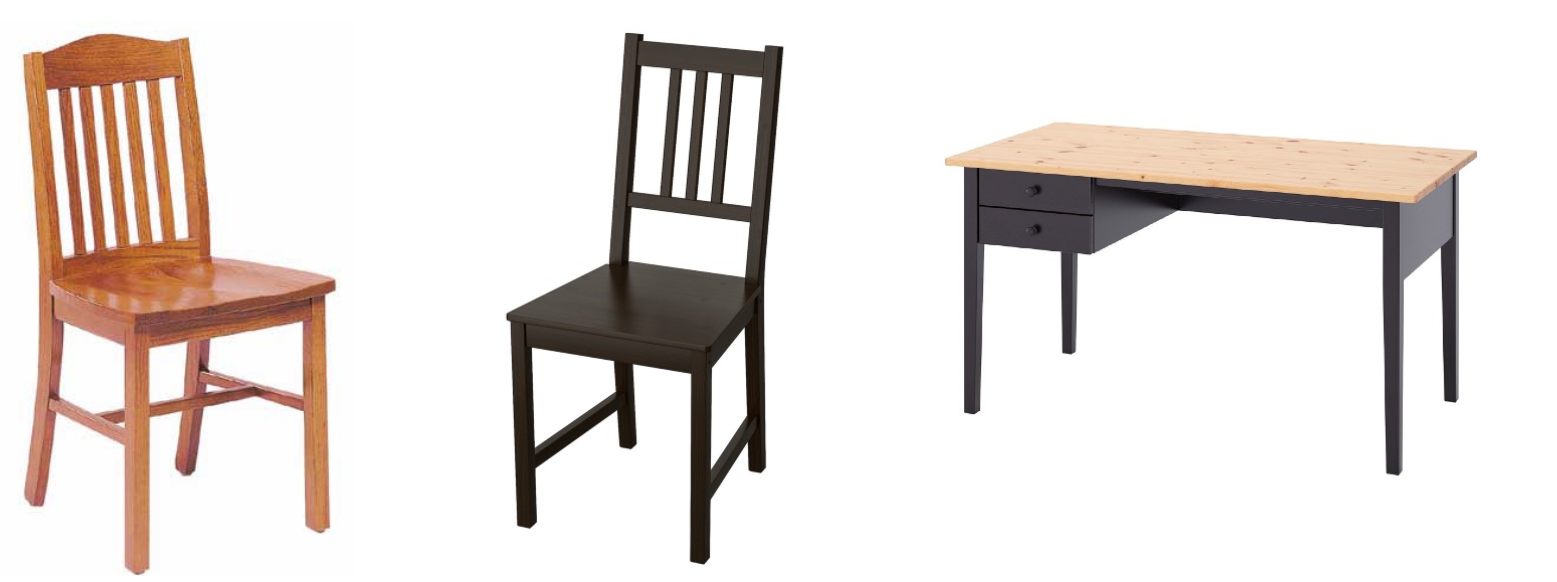
\includegraphics[width=4cm]{figures/1174086/chapter8/teori5.png}
                \centering
                  \caption{Teori No 5}
            \end{figure}

            \item apa itu adversarial play
            \par adversarial play adalah dimana para jaringan di latih, dimana jaringan satu dan lainnya saling berkompetisi. dapat disimpulkan dimana jaringan generator dan jaringan discriminator saling bertemu berulang ulang kali
            
            \item Jelaskan dengan ilustrasi gambar apa itu Nash equilibrium
            \par Nash equilibrium adalah konsep dalam teori permainan di mana hasil optimal dari permainan adalah di mana tidak ada insentif untuk menyimpang dari strategi awal mereka. Lebih khusus lagi, keseimbangan Nash adalah konsep teori permainan di mana hasil optimal dari permainan adalah di mana tidak ada pemain yang memiliki insentif untuk menyimpang dari strategi yang dipilihnya setelah mempertimbangkan pilihan lawan.
            \begin{figure}[H]
                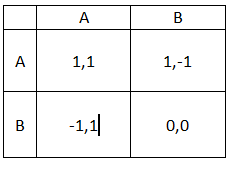
\includegraphics[width=4cm]{figures/1174086/chapter8/teori7.png}
                \centering
                  \caption{Teori No 7}
            \end{figure}

            \item Sebutkan dan jelaskan contoh-contoh implementasi dari GAN
            \par Pada bidang mode, seni, dan iklan, GAN dapar digunakan untuk membuat foto-foto model fashion imajinier tanpa perlu menyewa model. Pada bidang sains GAN dapat meningkatkan citra astronomi dan mensimulasikan pelensaan gravitasi untuk penelitian materi gelap.

            \item Berikan contoh dengan penjelasan kode program beserta gambar arsitektur untuk membuat generator(neural network) dengan sebuah input layer, tiga hidden layer(dense layer), dan satu output layer(reshape layer)
\begin{verbatim}
gen=Sequential() #Inisiasi dari sequensial
gen.add(Dense(units=200,input\_dim=np.shape(train\_input)[1])) #Menambah dense layer dengan batch size 200 dan input dim dari input
gen.add(Dense(units=400))#Menambah dense layer dengan batch size 400 dan input dim 100
gen.add(Dense(units=784, activation='tanh')) #Menambah dense layer dengan batch size 784 dan aktivasi metode tanh
gen.compile(loss='binary\_crossentropy', optimizer=adam\_optimizer()) #Menkompilasi hasil penambahan setiap dense
 gen.summary() #Memproses data yang sudah disetting dan menampilkannya
\end{verbatim}    
            \par Pada contoh tersebut, data akan diambil dari hasil proses sebelumnya yaitu proses ekstrasi data gambar. Dari contoh ini, terdapat 3 layer dense, 1 input layer dan 1 output layer. Dari input layer nanti akan dimasukkan terlebih dahulu ke dense layer pertama lalu diproses oleh 2 layer selanjutnya dan terakhir akan ditampilkan oleh layer output.
            \begin{figure}[H]
                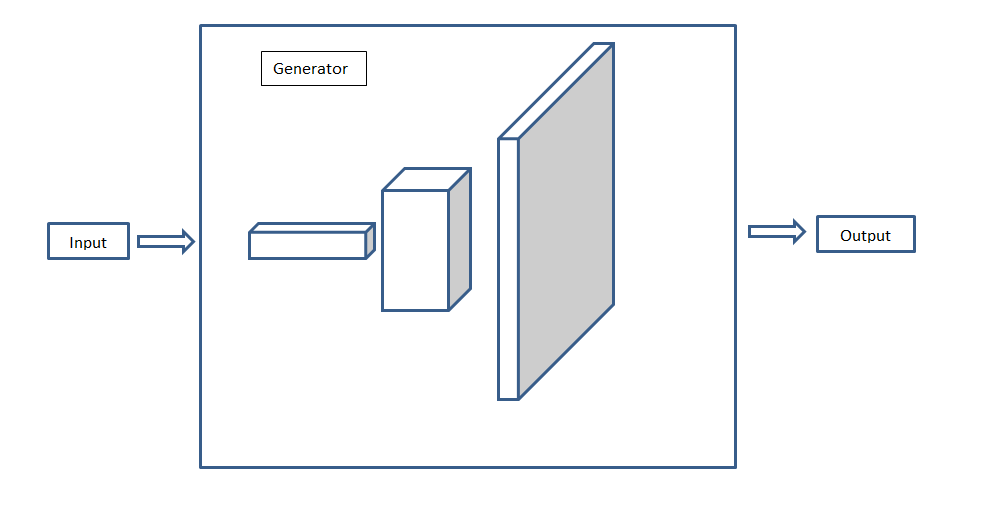
\includegraphics[width=4cm]{figures/1174086/chapter8/teori9.png}
                \centering
                  \caption{Teori No 9}
            \end{figure}

            \item Berikan contoh dengan ilustrasi dari arsitektur dikriminator dengan sebuath input layer, 3 buah hidden layer, dan satu output layer.
\begin{verbatim}
diskrim=Sequential()#Inisiasi dari sequensial
diskrim.add(Dense(units=784,input\_dim=np.shape(train\_input)[1]))#Menambah dense layer dan input dim dari layer
diskrim.add(Dense(units=400)) #Mensetting Dense
diskrim.add(Dense(units=200, activation='sigmoid')) #Mensetting dense dan melakukan aktivasi dengan metode sigmoid
diskrim.compile(loss='binary\_crossentropy', optimizer=adam\_optimizer())#Menkompilasi hasil penambahan setiap dense
diskrim.summary()#Memproses data yang sudah disetting dan menampilkannya
\end{verbatim}
            \par Pada contoh tersebut, data akan diambil dari hasil proses sebelumnya yaitu proses ekstrasi data gambar. Dari contoh ini, terdapat 3 layer dense, 1 input layer dan 1 output layer. Pada proses ini, seluruh data akan dibandingkan dengan data sebelumnya yaitu dari generator dan dari data aslinya yang sudah dijadikan data vector. 
            \begin{figure}[H]
                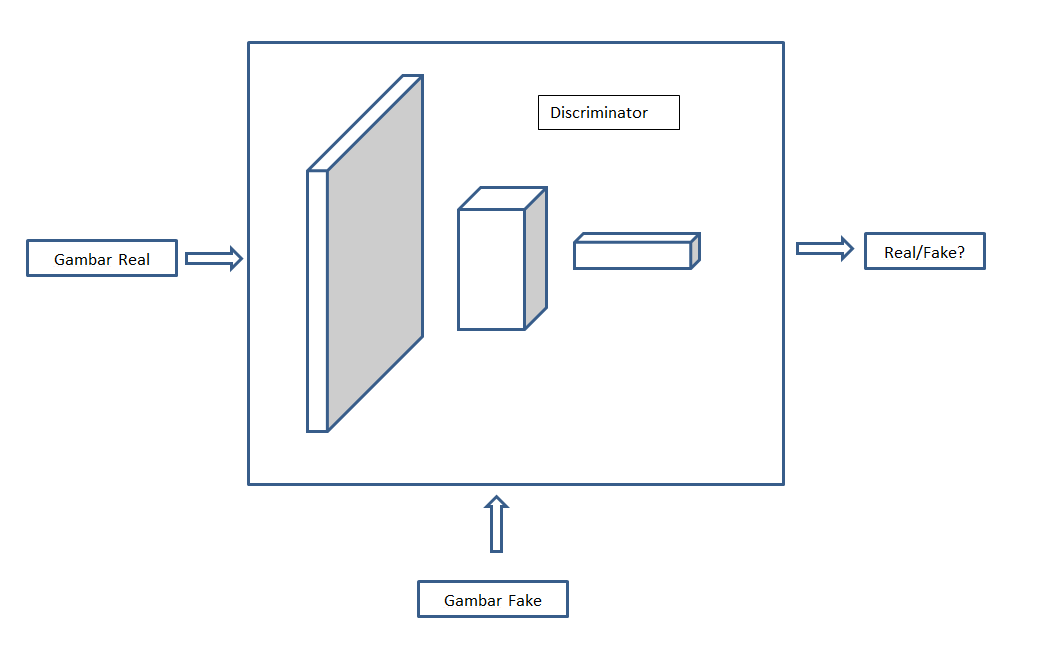
\includegraphics[width=4cm]{figures/1174086/chapter8/teori10.png}
                \centering
                  \caption{Teori No 10}
            \end{figure}
            
            \item Jelaskan bagaimana kaitan output dan input antara generator dan diskriminator tersebut. Jelaskan kenapa inputan dan outputan seperti itu
            \par Pada kedua metode tersebut, akan disebutkan berapa akurasi dari setiap metode. Pada setiap metode tersebut (Discriminator dan generator) akan dilakukan pelatihan dan akan dibandingkan hasilnya. Generator akan menghasilkan data baru sesuai dengan hasil latihan dan dari data tersebut, discriminator akan membandingkan dengan data set apakah data tersebut "asli" atau tidak.
            
            \item Jelaskan apa perbedaan antara Kullback-Leibler divergence (KL divergence)/relative entropy, Jensen-Shannon(JS) divergence / information radius(iRaD) / total divergence to the average dalam mengukur kualitas dari model
            \par relative entropy adalah ukuran dari bagaimana satu distribusi probabilitas berbeda dari yang kedua, distribusi probabilitas referensi, Divergensi Jensen-Shannon adalah ukuran divergensi berprinsip yang selalu terbatas untuk variabel acak terbatas.

            \item Jelaskan apa itu fungsi objektif yang berfungsi untuk mengukur kesamaan antara gambar yang dibuat dengan yang asli.
            \par Fungsi objektif adalah fungsi yang digunakan sebagai penujuk berapa nilai kesamaan anatara gambar yang dibuat dengan yang asli

            \item Jelaskan apa itu scoring algoritma selain mean square error atau cross entropy seperti The Inception Score dan The Frechet Inception distance.
            \par Inception Score digunakan untuk mengukur seberapa realistis output dari GAN, dimana ada dua parameter, yaitu : gambarnya punya variasi dan setiap gambar jelas terlihat seperti sesuatu. Frechet Inception Distance adalah ukuran kesamaan antara dua dataset gambar. Itu terbukti berkorelasi baik dengan penilaian manusia terhadap kualitas visual dan paling sering digunakan untuk mengevaluasi kualitas sampel Generative Adversarial Networks. FID dihitung dengan menghitung jarak Fréchet antara dua Gaussians dipasang ke representasi fitur dari jaringan Inception.
            
            \item Jelaskan kelebihan dan kekurangan GAN
            \begin{itemize}
              \item Kelebihan 
              \begin{enumerate}
               
                \item GAN Menghasilkan data baru yang bisa hampir mirip dengan data asli. Karena hasil pelatihannya, GAN dapat menghasilkan data gambar, teks, audio, dan video yang dapat dibilang hampir mirip dengan yang aslinya. Berkat hal tersebut, GAN dapat digunakan dalam sistem marketing, e-commerce, games,iklan, dan industri lainnya
                \item GAN mempelajari representasi data secara internal sehingga beberapa masalah pada machine learning dapat diatasi dengan mudah
                \item Discriminator yang sudah dilatih dapat menjadi sebuah classifier atau pendeteksi jika data sudah sesuai. Karena Discriminator yang akan menjadi tidak efisien berkat seringnya dilatih
                \item GAN dapat dilatih menggunakan data yang belum dilabeled
              
            \end{enumerate}
              \item Kekurangan
              \begin{enumerate}  
                \item Data saat diproses oleh metode gan tidak konvergensi
                \item Jenis sampel yang dihasilkan oleh generator terbatas karena modenya terbatas
                \item Ketidak seimbangnya antara generator dan discriminator dapat menyebabkan overfitting atau terlalu dekat dengan hasil sampel
                \item Sangat sensitif dengan data yang sudah diinisiasi sebelumnya
              \end{enumerate}
            \end{itemize}

        \end{enumerate}

        \subsection{Praktek}
        \begin{enumerate}
        \item Jelaskan apa itu 3D convolutions
        Konvolusi 3D. Konvolusi 3D menerapkan filter 3 dimensi ke dataset dan filter bergerak 3 arah (x, y, z) untuk menghitung representasi fitur level rendah. Bentuk output mereka adalah ruang volume 3 dimensi seperti kubus atau kuboid.
        
        \item Jelaskan dengan kode program arsitektur dari generator networknya, beserta penjelasan input dan output dari generator network.
        \lstinputlisting{src/1174086/chapter8/no2.py}
        generator ialah g\_loss, Bentuk jaringan Generator dapat dilihat berkebalikan dengan struktur jaringan saraf pada umumnya. Jaringan Generator menerima input sebuah vektor angka z, kemudian mengubahnya menjadi output gambar tiga dimensi.
        
        \item Jelaskan dengan kode program arsitektur dari diskriminator network, beserta penjelasan input dan outputnya.
        \lstinputlisting{src/1174086/chapter8/no3.py}
        diskrimanator adalah d\_loss, Jaringan Discriminator merupakan jaringan klasifikasi biner yang menerima input gambar tiga dimensi dan mengeluarkan klasifikasi menyatakan input gambar adalah gambar asli dari dataset atau merupakan gambar buatan Generator.
        
        \item Jelaskan proses training 3D-GANs
        proses training 3D gan yaitu dengan melakukan epoch sebanyak yang ditentukan.
        
        \item Jelaskan bagaimana melakukan settingan awal chapter 02 untuk memenuhi semua kebutuhan sebelum melanjutkan ke tahapan persiapan data.
        1. clone github										 2. download dataset 									3. buat folder baru logs dan results
        
        \item Jelaskan tentang dataset yang digunakan, dari mulai tempat unduh, cara membuka dan melihat data. Sampai deskripsi dari isi dataset dengan detail penjelasan setiap folder/file yang membuat orang awam paham.
        dataset digunakan yaitu 3DShapeNets yang berisi model model bentuk benda dll, folder train berisi train dan folder test berisi data testing. dan semua data tersebut di simpan didalam folder volumetric\_data 
        
        \item Jelaskan apa itu voxel dengan ilustrasi dan bahasa paling awam
        Volume pixel atau voxel adalah titik dalam ruang tiga dimensi. Sebuah voxel mendefinisikan posisi dengan tiga koordinat dalam arah x, y, dan z. Sebuah voxel adalah unit dasar untuk mewakili gambar 3D
        
        \item Visualisasikan dataset tersebut dalam tampilan visual plot, jelaskan cara melakukan visualisasinya
        1. import library									   2. load data file .mat  								  3. lalu read memakai matplotlib
        
        \item buka file run.py jelaskan perbaris kode pada fungsi untuk membuat generator yaitu build generator.
        membuat generator yaitu dengan ketentukan gen sebagai variabel dan membuat fungsi atau variabel gen\_model lalu dilakukan return
        
        \item jelaskan juga fungsi untuk membangun diskriminator pada fungsi build discriminator.
        membangun diskriminator berfungsi untuk mendefenisikan seluruh gambar yang sudah di load generator sebagai gambar fake dan real
        
        \item Jelaskan kode program
        \lstinputlisting{src/1174086/chapter8/1.py}
        Jika interpreter python menjalankan if name main  sebagai program utama, itu ialah menetapkan variabel name  untuk memiliki nilai main. Jika file ini sedang diimpor dari modul lain, name akan ditetapkan ke nama modul. Nama modul tersedia sebagai nilai untuk name variabel global.
        
        \item Jelaskan kode program 
        \lstinputlisting{src/1174086/chapter8/2.py}
        artinya adalah load dataset yang hanya dalam folder chair data train
        
        \item Jelaskan kode program 
        \lstinputlisting{src/1174086/chapter8/3.py}
        disini menggunakan Adam sebagai algoritma pengoptimalan dan binary\_crossentropy sebagai kerugian loss. 
        
        \item Jelaskan kode program 
        \lstinputlisting{src/1174086/chapter8/4.py}
        ini artinya ialah kita memasukkan random vector kedalam generator model lalu membagi 2 yaitu generated example dan real example, dan meneruskan ke diskriminator model sebagai real atau fake
        
        \item Jelaskan kode program 
        \lstinputlisting{src/1174086/chapter8/5.py}
        ini melakukan load data pada dataset
        
        \item Jelaskan kode program 
        \lstinputlisting{src/1174086/chapter8/6.py}
        ini berfungsi untuk membuat tensorboard yang nantinya bisa diakses melalui localhost
        
        \item Jelaskan kode program 
        \lstinputlisting{src/1174086/chapter8/7.py}
        fungsi ini ialah untuk melakukan reshape agar shape yang dihasilkan tidak terlalu besar.
        
        \item Jelaskan kode program 
        \lstinputlisting{src/1174086/chapter8/8.py}
        karena jika epoch semakin banyak maka kualiatas training yang dihasilkan akan semakin baik
        
        \item Jelaskan kode program 
        \lstinputlisting{src/1174086/chapter8/9.py}
        batch adalah jumlah file yang akan di training
        
        \item Jelaskan kode program 
        \lstinputlisting{src/1174086/chapter8/10.py}
        ini adalah untuk membuat gambar bersih dari noise dan juga menyesuaikan shape
        
        \item Jelaskan kode program 
        \lstinputlisting{src/1174086/chapter8/11.py}
        ialah membuat sample gambar palsu yang akan diteruskan ke diskriminator
        
        \item Jelaskan kode program 
        \lstinputlisting{src/1174086/chapter8/12.py}
        diskriminator bisa load gambar fake dan real dari generator, oleh karena itu ada generator loss dan diskriminator loss untuk melihat seberapa baik kualitas yang dihasilkan
        
        \item Jelaskan kode program 
        \lstinputlisting{src/1174086/chapter8/13.py}
        dengan melakukan print g\_loss untuk generator dan juga d\_loss untuk diskriminator
        
        \item Jelaskan kode program 
        \lstinputlisting{src/1174086/chapter8/14.py}
        mengapa ada perulangan karena untuk melakukan perbandingan dari hasil yang sudah didapat.
        
        \item Jelaskan kode program 
        \lstinputlisting{src/1174086/chapter8/15.py}
        TensorBoard adalah sebuah aplikasi web localhost untuk memeriksa dan menyelesaikan grafik dari hasil TensorFlow.
        
        \item Jelaskan kode program 
        \lstinputlisting{src/1174086/chapter8/16.py}
        File H5 adalah file data yang disimpan dalam Format Data Hirarki (HDF). Ini berisi array multidimensi data ilmiah
        
        \item Jelaskan kode program 
        \lstinputlisting{src/1174086/chapter8/17.py}
        ini adalah tahap akhir untuk melakukan testing dari model yang telah dibuat dan buat model dari yang sudah di create sebelumnya yaitu generator dan diskriminator.
        
        \begin{figure}[H]
        \centering
        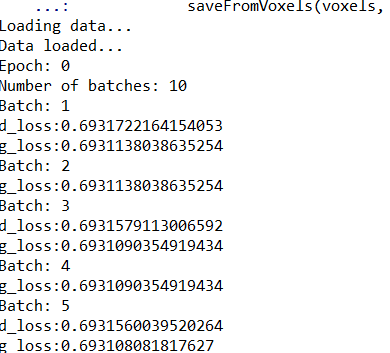
\includegraphics[width=4cm]{figures/1174086/chapter8/1.png}
        \caption{Result}
        \end{figure}
        
        \begin{figure}[H]
        \centering
        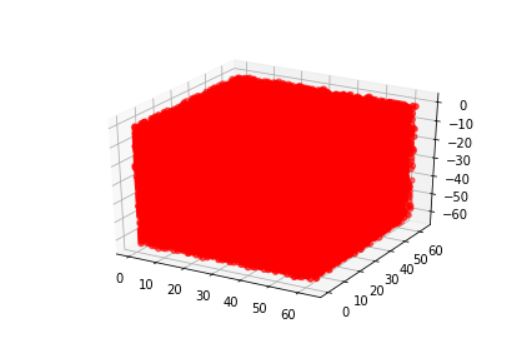
\includegraphics[width=4cm]{figures/1174086/chapter8/2.png}
        \caption{Result} 
        \end{figure}
        
        \begin{figure}[H]
          \centering
          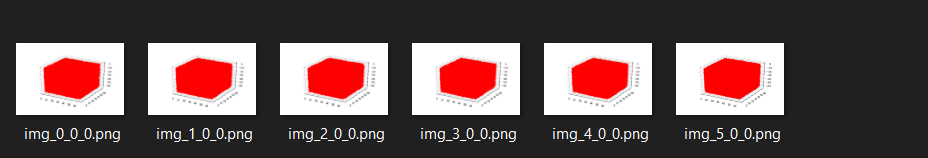
\includegraphics[width=4cm]{figures/1174086/chapter8/3.png}
        \caption{Result}
 
        \end{figure}
        
        \begin{figure}[H]
        \centering
        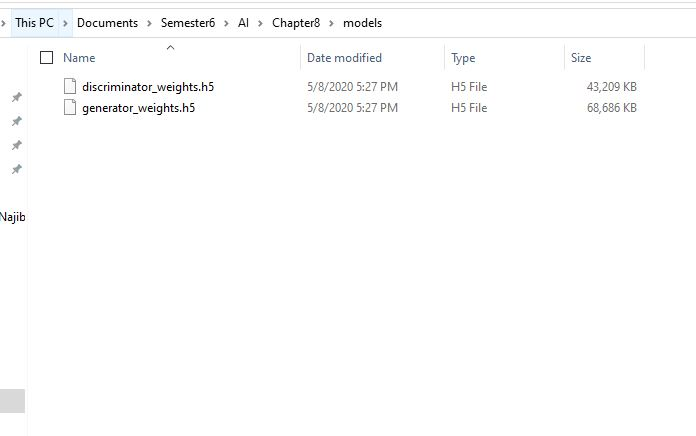
\includegraphics[width=4cm]{figures/1174086/chapter8/4.jpg}
        \caption{Result}
        \end{figure}
        
        
        \end{enumerate}
